
\documentclass[11pt]{article}
\usepackage[margin=0.78in]{geometry}
\usepackage{booktabs}
\usepackage{graphicx}
\usepackage{float}
\usepackage{hyperref}
\hypersetup{colorlinks=true, linkcolor=blue, urlcolor=blue}
\title{Conservative Transformer Floor Selection Report}
\author{SPY American Call TP2 Project}
\date{\today}
\begin{document}
\maketitle

\section{Purpose}
This report evaluates the corrected-history TP2-MV-ALiBi transformer with conservative probability-floor risk controls. The transformer still tunes its exact threshold on validation P\&L, but the threshold cannot fall below a fixed floor. To avoid relying on one hand-picked value, we report floors 0.10, 0.20, and 0.30 side by side. The 0.20 floor is treated as the primary moderate rule; 0.10 and 0.30 are robustness checks.

\section{Leakage Control}
The floor family is treated as a risk-control design choice. Within each rolling fold and each fixed floor, the exact threshold is selected using the validation year only. The test year is evaluated once. No test-year P\&L enters threshold tuning.

\section{Aggregate Results Across Fixed Floors}
\begin{table}[H]
\centering
\small
\begin{tabular}{rrrrrrr}
\toprule
Floor & Trades & P\&L & Positive years & Sharpe & Sortino & Max DD \\
\midrule
0.10 & 69,679 & \$5,818,061 & 5/6 & 1.21 & 5.21 & -\$1,863,540 \\
0.20 & 43,123 & \$6,413,690 & 6/6 & 1.76 & 8.14 & -\$735,990 \\
0.30 & 26,497 & \$3,283,189 & 6/6 & 1.85 & 6.44 & -\$286,855 \\
\bottomrule
\end{tabular}
\end{table}

\begin{figure}[H]
\centering
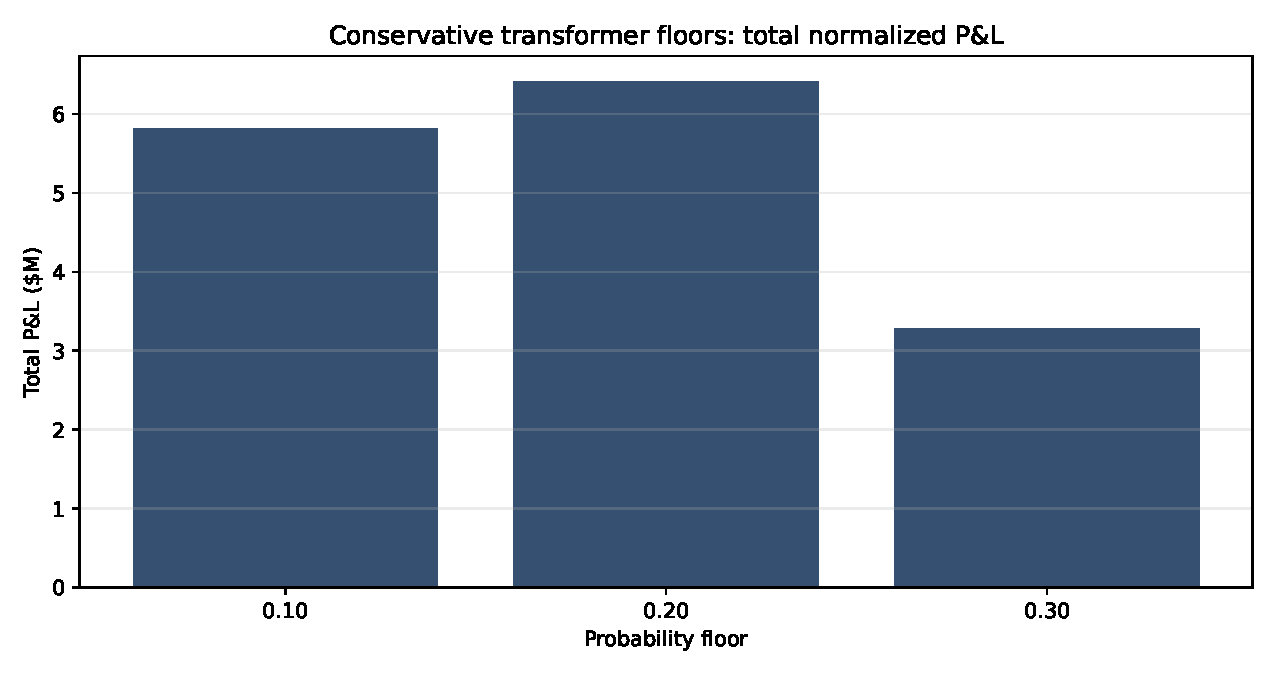
\includegraphics[width=0.82\linewidth]{figures/conservative_transformer_floor_summary_pnl.pdf}
\caption{Total normalized P\&L for the fixed confidence-floor family.}
\end{figure}

\section{Primary Floor Yearly Results}
The table below reports the primary moderate floor, \(p \geq 0.20\). The adjacent floors are retained in the aggregate robustness table above.

\begin{table}[H]
\centering
\small
\begin{tabular}{rrrrrrr}
\toprule
Year & Threshold & Trades & P\&L & Sharpe & Sortino & Max DD \\
\midrule
2021 & 0.20 & 15382 & \$3,339,496 & 2.12 & 9.74 & -\$735,990 \\
2022 & 0.53 & 717 & \$23,338 & 1.16 & 0.80 & -\$26,372 \\
2023 & 0.42 & 2106 & \$12,829 & 0.80 & 0.99 & -\$34,941 \\
2024 & 0.20 & 11629 & \$304,278 & 1.27 & 2.22 & -\$470,283 \\
2025 & 0.20 & 12212 & \$2,127,171 & 2.16 & 23.38 & -\$163,421 \\
2026 & 0.20 & 1077 & \$606,577 & 2.88 & 231.14 & -\$12,613 \\
\bottomrule
\end{tabular}
\end{table}

\begin{figure}[H]
\centering
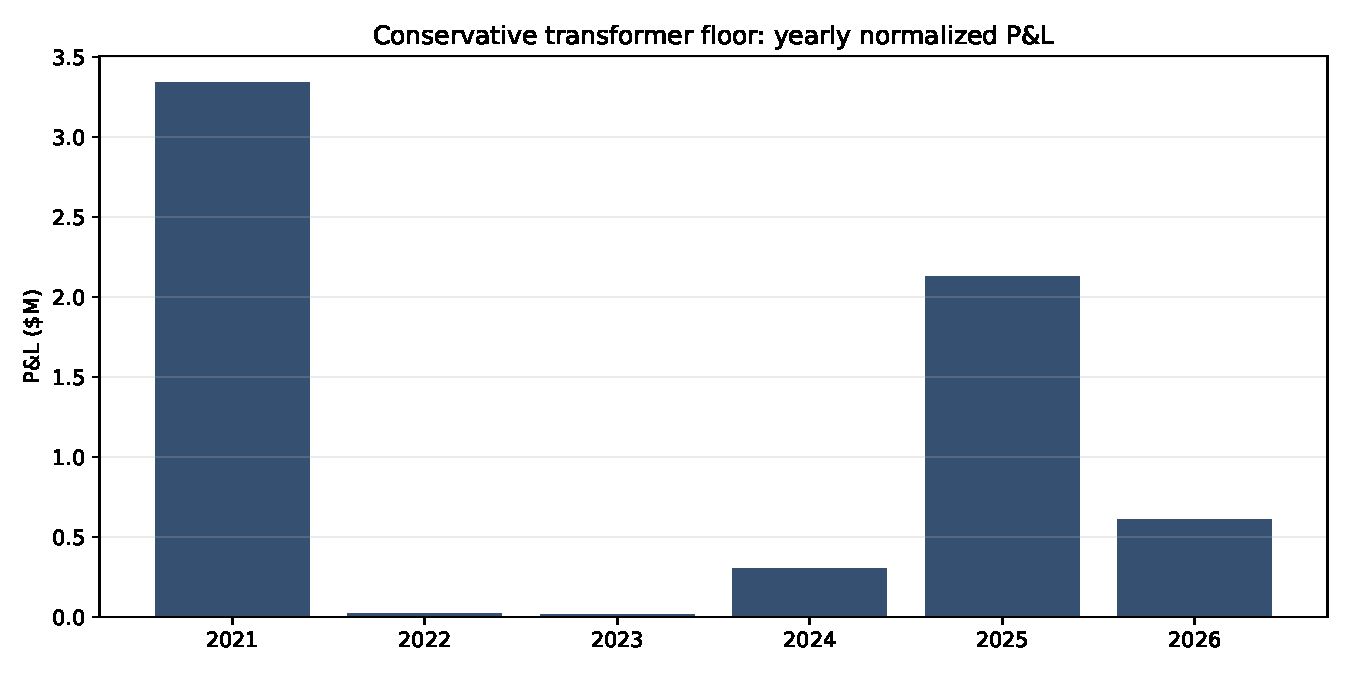
\includegraphics[width=0.88\linewidth]{figures/conservative_transformer_floor_yearly_pnl.pdf}
\caption{Yearly normalized P\&L under the conservative transformer floor rule.}
\end{figure}

\begin{figure}[H]
\centering
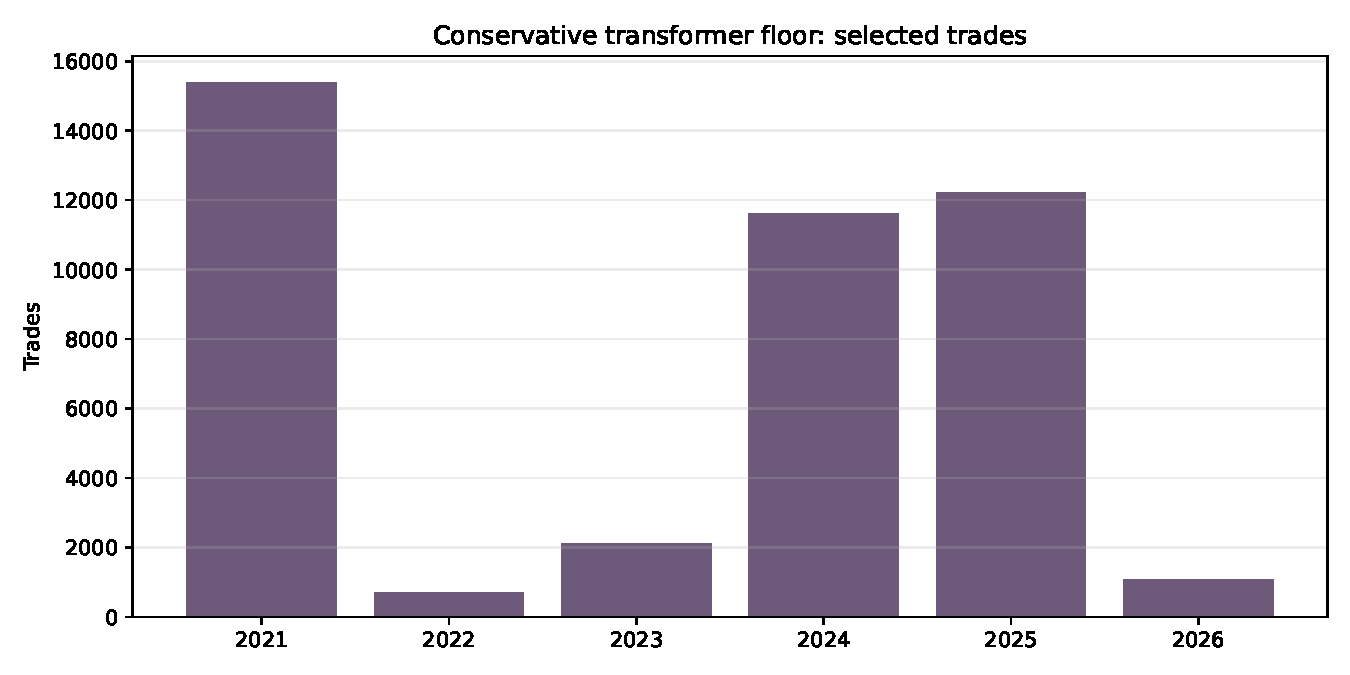
\includegraphics[width=0.88\linewidth]{figures/conservative_transformer_floor_trades.pdf}
\caption{Selected trade counts under the conservative transformer floor rule.}
\end{figure}

\section{Interpretation}
The raw transformer selected too many low-confidence trades in adverse years. The conservative floor reduces over-selection by requiring a minimum model confidence before any trade can enter. This should be presented as a risk-control layer, not as a new arbitrage condition.

\end{document}
